\hypertarget{interface_t_p_parameter_chart_color}{
\section{TPParameterChartColor Class Reference}
\label{interface_t_p_parameter_chart_color}\index{TPParameterChartColor@{TPParameterChartColor}}
}
{\tt \#import $<$TPParameterChartColor.h$>$}

Inheritance diagram for TPParameterChartColor::\begin{figure}[H]
\begin{center}
\leavevmode
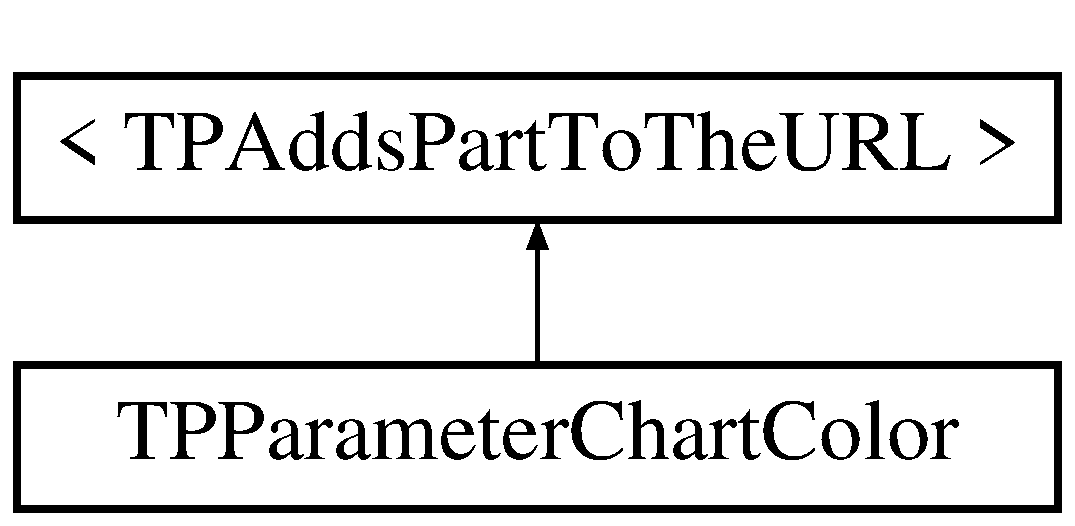
\includegraphics[height=2cm]{interface_t_p_parameter_chart_color}
\end{center}
\end{figure}
\subsection*{Public Member Functions}
\begin{CompactItemize}
\item 
(void) - \hyperlink{interface_t_p_parameter_chart_color_21f439b808b2f6a9495c337e740db7b8}{setColors:}
\end{CompactItemize}


\subsection{Detailed Description}
This class is responsible for controlling which data has what color 

\subsection{Member Function Documentation}
\hypertarget{interface_t_p_parameter_chart_color_21f439b808b2f6a9495c337e740db7b8}{
\index{TPParameterChartColor@{TPParameterChartColor}!setColors:@{setColors:}}
\index{setColors:@{setColors:}!TPParameterChartColor@{TPParameterChartColor}}
\subsubsection[{setColors:}]{\setlength{\rightskip}{0pt plus 5cm}- (void) setColors: (NSArray $\ast$) {\em colors}}}
\label{interface_t_p_parameter_chart_color_21f439b808b2f6a9495c337e740db7b8}


set the colors \begin{Desc}
\item[Parameters:]
\begin{description}
\item[{\em colors}]NSArray with \hyperlink{interface_t_p_color}{TPColor} objects \end{description}
\end{Desc}


The documentation for this class was generated from the following files:\begin{CompactItemize}
\item 
TPParameterChartColor.h\item 
TPParameterChartColor.m\end{CompactItemize}
